\section{Validation and Verification}
\subsection{Software in the loop}
This section describe the software in the loop infrastructure and test procedure for the IMU driver. This is as follow:
\begin{itemize}
    \item The tester allocate two device files to simulate virtual serial port.
    \item The tester starts the software in the loop application. The application immediately starts to write fake imu measurements data to the virtual device file.
    \item The tester starts the test (dummy) application that contains the driver. The driver application reads data from the virtual device file.
    \item The test application process the IMU message and determine if the test is a success or failure depending on the content.
\end{itemize}



\begin{figure}[ht]
    \centering
    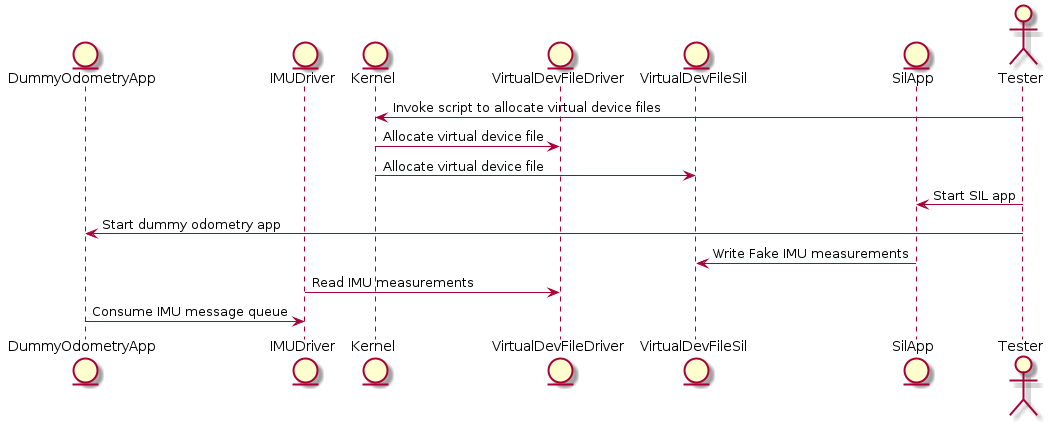
\includegraphics[width=0.75 \textwidth]{diagrams/software_in_the_loop.png}
    \caption{High level overview of SIL test procedure}
    \label{reference}
\end{figure}
